% !TeX root = chapter_dippsApplications.Rnw

\documentclass[tikz]{standalone}
 
\usetikzlibrary{positioning}
\usetikzlibrary{calc}
 
% \newcommand{\refsec}{{\color{red}SecRef}}
% \newcommand{\reffig}{{\color{red}FigRef}}
 
\begin{document}
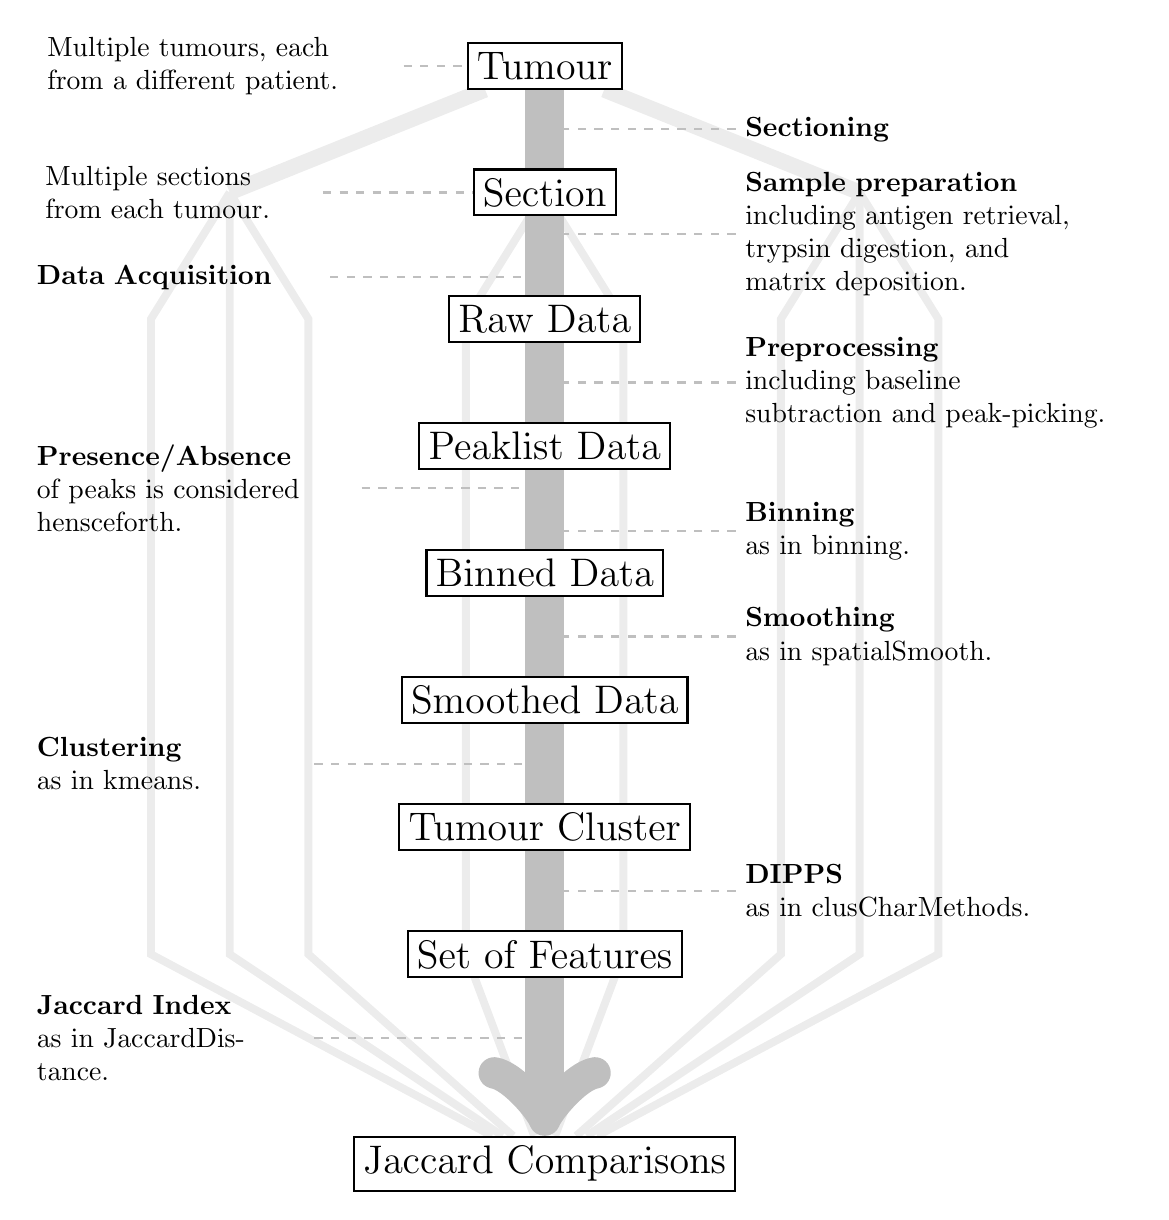
\begin{tikzpicture}

% \begin{scope}[on grid]

% \draw[help lines,step=5mm,gray!20] (5,-5) grid (17,12);





%%% Initialise Nodes
\draw (10,10) node[draw,thick] (a) {{\Large Tumour }};
\node[draw,below=1cm of a,thick] (b) {{\Large Section}};
\node[draw,below=1cm of b,thick] (c) {{\Large Raw Data }};
\node[draw,below=1cm of c,thick] (d) {{\Large Peaklist Data }};
\node[draw,below=1cm of d,thick] (e) {{\Large Binned Data }};
\node[draw,below=1cm of e,thick] (f) {{\Large Smoothed Data }};
\node[draw,below=1cm of f,thick] (g) {{\Large Tumour Cluster }};
\node[draw,below=1cm of g,thick] (h) {{\Large Set of Features}};
\node[draw,below=2cm of h,thick] (i) {{\Large Jaccard Comparisons }};

%%% Flow Lines
% Patient B
\draw[line width = 2mm, gray!15] (a) -- ($(b) - (4,0)$);
\draw[line width = 1mm, gray!15] ($(b) - (4,0)$) -- ($(c) - (5,0)$) -- ($(h) - (5,0)$) -- (i);
\draw[line width = 1mm, gray!15] ($(b) - (4,0)$) -- ($(c) - (4,0)$) -- ($(h) - (4,0)$) -- (i);
\draw[line width = 1mm, gray!15] ($(b) - (4,0)$) -- ($(c) - (3,0)$) -- ($(h) - (3,0)$) -- (i);
% Patient C
\draw[line width = 2mm, gray!15] (a) -- ($(b) + (4,0)$);
\draw[line width = 1mm, gray!15] ($(b) + (4,0)$) -- ($(c) + (5,0)$) -- ($(h) + (5,0)$) -- (i);
\draw[line width = 1mm, gray!15] ($(b) + (4,0)$) -- ($(c) + (4,0)$) -- ($(h) + (4,0)$) -- (i);
\draw[line width = 1mm, gray!15] ($(b) + (4,0)$) -- ($(c) + (3,0)$) -- ($(h) + (3,0)$) -- (i);
% Patient A
\draw[line width = 1mm, gray!15] (b) -- ($(c) - (1,0)$) -- ($(h) - (1,0)$) -- (i);
\draw[line width = 1mm, gray!15] (b) -- ($(c) + (1,0)$) -- ($(h) + (1,0)$) -- (i);
\draw[->,line width = 5mm, gray!50] (a) -- (i);

%%% Re-Initialise Nodes (draw over flow-lines)
\draw (10,10) node[draw,thick,fill=white] {{\Large Tumour }};
\node[draw,below=1cm of a,thick,fill=white] {{\Large Section}};
\node[draw,below=1cm of b,thick,fill=white] {{\Large Raw Data }};
\node[draw,below=1cm of c,thick,fill=white] {{\Large Peaklist Data }};
\node[draw,below=1cm of d,thick,fill=white] {{\Large Binned Data }};
\node[draw,below=1cm of e,thick,fill=white] {{\Large Smoothed Data }};
\node[draw,below=1cm of f,thick,fill=white] {{\Large Tumour Cluster }};
\node[draw,below=1cm of g,thick,fill=white] {{\Large Set of Features}};
\node[draw,below=2cm of h,thick,fill=white] {{\Large Jaccard Comparisons }};



%% Comments and Notes
\node[left=0.8cm of a,text width = 4.4cm] (n1) {Multiple tumours, each from a different patient.};
\draw[dashed,gray!50,thick] (n1) -- (a);

\node[left=1.9cm of b,text width = 3.4cm] (n2) {Multiple sections from each tumour.};
\draw[dashed,gray!50,thick] (n2) -- (b);

\draw ($ (a) !.5! (b) $) node (ab) {};
\node[right=2.3cm of ab] (s1) {{\bf Sectioning }};
\draw[dashed,gray!50,thick] (s1) -- (ab);

\draw ($ (b) !.33! (c) $) node (bc) {};
\node[right=2.3cm of bc, text width = 4.9cm] (s2) {{\bf Sample preparation} \\ including antigen retrieval, trypsin digestion, and \\ matrix deposition.};
\draw[dashed,gray!50,thick] (s2) -- (bc);
\draw ($ (b) !.67! (c) $) node (bc2) {};
\node[left=2.6cm of bc2, text width = 3.6cm] (s2) {{\bf Data Acquisition }};
\draw[dashed,gray!50,thick] (s2) -- (bc2);

\draw ($ (c) !.5! (d) $) node (cd) {};
\node[right=2.3cm of cd,text width = 4.9cm] (s3) {{\bf Preprocessing } \\ including baseline \\ subtraction and peak-picking.};
\draw[dashed,gray!50,thick] (s3) -- (cd);

\draw ($ (d) !.33! (e) $) node (de) {};
\node[left=2.2cm of de, text width = 4cm] (s4) {{\bf Presence/Absence } \\ of peaks is considered hensceforth.};
\draw[dashed,gray!50,thick] (s4) -- (de);

\draw ($ (d) !.67! (e) $) node (de2) {};
\node[right=2.3cm of de2, text width = 4.9cm] (s5) {{\bf Binning } \\ as in \refapp{binning}.};
\draw[dashed,gray!50,thick] (s5) -- (de2);


\draw ($ (e) !.5! (f) $) node (ef) {};
\node[right=2.3cm of ef, text width = 4.9cm] (s6) {{\bf Smoothing } \\ as in \refsec{spatialSmooth}.};
\draw[dashed,gray!50,thick] (s6) -- (ef);

\draw ($ (f) !.5! (g) $) node (fg) {};
\node[left=2.8cm of fg, text width = 3.4cm] (s7) {{\bf Clustering } \\ as in \refsec{kmeans}.};
\draw[dashed,gray!50,thick] (s7) -- (fg);

\draw ($ (g) !.5! (h) $) node (gh) {};
\node[right=2.3cm of gh, text width = 4.9cm] (s8) {{\bf DIPPS } \\ as in \refsec{clusCharMethods}.};
\draw[dashed,gray!50,thick] (s8) -- (gh);

\draw ($ (h) !.4! (i) $) node (hi) {};
\node[left=2.8cm of hi, text width = 3.4cm] (s9) {{\bf Jaccard Index } \\ as in \refsec{JaccardDistance}.};
\draw[dashed,gray!50,thick] (s9) -- (hi);



% \end{scope}


\end{tikzpicture}
\end{document}


